% TODO
\tdi{Voir si citer Vandpoul et la fondation petzl sur les risques en montagne}

L'objectif de cette première partie est de présenter le contexte
métier dans lequel notre thèse s'inscrit, celui du secours en
montagne. Nous commencerons par présenter l'organisation de ce service
public puis nous nous focaliserons sur la question de la localisation
des victimes en montagne, question au centre de notre travail de
recherche.

\subsection{Organisations passées et présente du secours en montagne
  français}
\label{subsec:1-1-1}

\subsubsection{De la solidarité montagnarde à la mission régalienne}
\label{subsubsec:1-1-1-1}

L'organisation et le fonctionnement des \emph{secours en montagne}
contemporains est fortement influencé par les structures et les
organisations qui l'ont précédé. C'est pourquoi il nous a semblé
nécessaire de revenir sur l'histoire de ces dernières, afin de décrire
la longue mise en place des \emph{secours en montagne} français. Notre
objectif n'est cependant pas d'entreprendre un travail d'historien,
très éloigné de nos compétences et de l'objet de cette thèse, mais
d'apporter un éclairage, que nous souhaitons le plus complet possible,
sur ce service public \footnote{Les événements principaux décrits dans
  cette partie sont synthétisés par la figure
  \ref{fig:frise_chronologique}, page
  \pageref{fig:frise_chronologique}.}.

\paragraph{Le \enquote{proto-secours} en montagne}
\label{par:1-1-1-1-1}

Si l'histoire du secours en montagne est intimement liée à celle de
l'alpinisme et, plus généralement, du tourisme montagnard, on ne
saurait l'y réduire. La présence humaine en milieu montagneux, bien
qu'impactée par ces activités, y est bien antérieure, et les montagnes
jouent, depuis longtemps, aussi bien le rôle de refuges, que de points
de passage, de \enquote{synapses} \autocite[p. 337]{Brunet1992}. De
fait, les massifs montagneux et notamment les Alpes sont parcourus
depuis l'Antiquité et les marchands ou voyageurs en périls sont
secourus par les habitants de ces vallées reculées
\autocite{Mezin2016}.

Cependant, cette forme d'assistance est bien différente du secours en
montagne contemporain. D'une part, car les \emph{espaces concernés}
sont différents. La haute-montagne est, jusqu'au \bsc{xix}\up{e}
siècle, \emph{terra incognita,} et ni les voyageurs, ni les locaux ne
s'y aventurent. Les secours ne se déroulent donc que le long
d'itinéraires traversants et non sur des arêtes effilées ou à flanc de
parois exposées. D'autre par, car il n'existe aucune forme
d'organisation pérenne, les caravanes de secours se forment lorsque
nécessaire, sur la base du volontariat.

Le champ d'action du secours en montagne va changer avec l’émergence
du nouveau divertissement \enquote{\textins{d}es grands bourgeois
  britanniques} \autocite{Descamps2018}, l'alpinisme. L'objectif n'est
plus de fuir les massifs les plus denses et les pentes les plus
abruptes, mais de les approcher. La difficulté des secours augmente
avec l'ambition des ascensions, mais ils sont toujours effectués par
des volontaires, comme des guides locaux\footnote{La première des
  compagnies de guide est crée en 1821 à Chamonix. Il s'agit de la
  seule compagnie de guides créée avant 1850
  \autocite{ContributeursWikipedia2020b}.} ou des alpinistes présents
sur place, ultérieurement soutenus par les militaires des régiments
alpins\footnote{Les régiments alpins sont crées en 1888
  \autocite{Mezin2016}.}.

Toutefois, l'organisation de ce \enquote{proto-secours} en montagne
n'est pas exempte de problèmes. Dans le récit d'une opération de
secours publié en 1911, \textcite{Thomas1911} met en évidence le fait
que, sous couvert de solidarité, les motivations des volontaires sont
également pécuniaires. Ces derniers étant discrètement dédommagés par
la victime ou, lorsque les secours n'ont pu aboutir, par sa
famille. Cette forme de rémunération, couplée à l'absence d'une
institution organisatrice, favorise, selon \textcite{Thomas1911}, la
multiplication de caravanes concurrentes, ce qui favorise les
interventions peu préparées et la prise de risque, rendant les secours
plus dangereux et moins efficaces. \textcite{Thomas1911} conclu son
propos par un appel a la rationalisation des secours. Il conseille de
recourir à des petits groupes de secouristes préparés et entrainés,
plutôt qu'à des caravanes organisées à la hâte et composées de
dizaines de volontaires.

Ce problème sera, en partie, résolu avec le développement de
regroupements de secouristes, centralisant la prise de décision : les
\emph{comité de secours.} Le premier d'entre eux, \emph{les sauveteurs
  volontaires du Salève,} apparait en 1897 dans les pré-alpes
\autocite{CFDLD}, 14 ans avant l'article de \bsc{Thomas.} Mais cette
initiative sera reprise bien plus tardivement dans d'autres
régions. \textcite{Caille2016} explique cette précocité par la forte
pression touristique subie par la région à la fin du \bsc{xix}\up{e}
siècle.  Le second comité de secours en montagne est créé à Grenoble
en 1910 \autocite{CFDLD,Caille2016}. Quant à la majorité de ces
structures, elles voient le jour au tournant des années 30, avec,
notamment, la création d'un comité de secours à Annecy en 1928, à
Chamonix en 1929, à Briançon en 1932 ou à Pau en 1936 \autocite{CFDLD,
  Devies1946}.

Cette organisation des secours, basée sur l'action de comités locaux
et sans réelle coordination entre massifs, perdurera jusqu'à
l'après-guerre. Durant cette période l'armée sera la seule institution
publique à participer activement aux secours en montagne. Son action
ira même en se renforçant, notamment par le support direct
(personnels) et indirect (développement de matériel, formation) de
\emph{l'école de haute-montagne} \acp{ehm} créée en 1932 à Chamonix
\autocite{Mezin2016}.

Cependant, en 1946 \textcite{Devies1946} remet en cause cette
organisation. De son point de vue les différents comités locaux sont
une solution bien insuffisante aux problèmes du secours en montagne,
notamment comparé aux solutions mises en place en Suisse ou en
Autriche. \bsc{Devies} prône une centralisation de l'organisation des
secours, par le biais d'une institution chapeautant les différents
comités locaux et subventionnée par l'État.

\paragraph{Le début d'une organisation nationale}

Les propositions de \bsc{Devies} aboutissent en 1947, lorsqu'il prend
la tête de la nouvelle commission de secours de la fédération
française de montagne \acp{ffm} \footnote{La \ac{ffm} est
  officiellement créée deux ans plus tôt, en 1945.}. L'objectif de
cette nouvelle institution est, comme il le proposait en 1946, de
fédérer les différents commités locaux pour proposer des réponses plus
efficaces aux situations de crise. Cette organisation permettra la
mise en place de secours d'envergure, comme en 1948, lorsqu'une
centaine de secouristes participent au sauvetage de deux alpinistes
coincés dans la face sud, d'une verticalité extrême, du Pavé dans le
massif des Écrins \autocite{Romanaz2018} ou en 1949 lors du sauvetage
de l'Olan \autocite{Mollaret1993}. Cette commission dirigera également
les secours lors des crashs du \emph{Canadian Pilgrim} sur l'Obiou et
du \emph{Malabar Princess} sur le mont-Blanc en 1950
\autocite{CFDLD,Mollaret1993,SDSM2013}.

Cependant, cette organisation semi-professionnelle montrera rapidement
ses limites, principalement à cause de difficultés de financement
\footnote{Problème que \bsc{Devies} avait déjà soulevé dans son
  article de 1946 \autocite{Devies1946}}, de recrutement, mais
également à cause de la hausse de fréquentation des massifs Alpins
\autocite{CFDLD}. Mais c'est en 1956, avec \emph{l'affaire Vincendon
  et Henry,} que les autorités prirent conscience des limites de cette
organisation bénévole des secours en montagne.

Le 22 décembre 1956 deux étudiants passionnés d'alpinisme, Jean
Vincendon et François Henry, entament l’ascension du mont Blanc
\autocite{Ballu1997}. Les deux hommes cherchent l'exploit, à une
époque où l'alpinisme hivernal est encore balbutiant. Ils décident
cependant de redescendre vers Chamonix et d'abandonner leur ascension
le 24, par crainte du mauvais temps à venir. Cependant, leur rencontre
avec la cordée du guide italien Walter Bonatti, déjà auréolé
d'ascensions notables comme la première du K2 en 1954
\footnote{Bonatti ne fera cependant pas partie des deux alpinistes
  ayant atteint le sommet \autocite{ContributeursWikipedia2020a}.} ou
l'ouverture en solitaire d'une voie dans la face sud-ouest des Drus en
1955 \footnote{Cette ascension n'est pas la première de la face ouest
  des Drus, celle-ci ayant été effectuée trois ans auparavant
  \autocite{ContributeursWikipedia2020}. Cependant l'ouverture en
  solitaire par \bsc{Bonatti} d'une voie au centre de la paroi et
  considérablement plus exposée est considérée comme l'une des plus
  importantes réalisations de l'alpinisme, qualifiée
  \enquote{\textins{d'}exploit magnifique et inspiré} par
  \textcite{Robbins2000}.}, les incite à reprendre l’ascension. Les
deux cordées, fidèles à leur itinéraire initial, se séparent le
lendemain. Bien qu'empruntant des itinéraires distincts, les deux
groupes se font surprendre par la nuit et bivouaquent sous la
tempête. Le lendemain Bonatti et son client atteignent le refuge
Vallot, alors que Vincendon et Henry, épuisés, prennent la décision de
descendre directement. Lors de la descente les deux alpinistes se
perdent et se retrouvent coincés sur une \gls{vire}. Exténués et
surchargés de matériel, ils sont incapables de rebrousser chemin et
passent une seconde nuit dehors.

Dans la vallée, les secours, prévenus dès le 25 décembre par un
proche, tardent à se mettre en place. La société chamoniarde de
secours en montagne, regroupant l'\ac{ehm}, la compagnie des guides de
Chamonix et de l'école nationale de ski alpin, n'arrive pas à
organiser une opération de secours, les guides refusant de s'aventurer
en haute-montagne en plein hiver et en pleine tempête. C'est
finalement l'\ac{ehm} qui prendra la direction des secours. Un premier
hélicoptère militaire est envoyé le 27 décembre, sans résultat, mais
les alpinistes sont repérés, à la longue-vue, un peu plus tard. La
configuration spatiale de l'événement favorise l'effervescence
médiatique, les accidentés étant visibles depuis Chamonix. De nombreux
médias nationaux, tels que la radio \emph{Europe 1,} nouvellement
créée, commencent à couvrir l'événement, et les secouristes doivent
opérer sous une pression médiatique alors inédite.

Les victimes étant localisées, une opération de secours héliportée est
organisée le 28 décembre. Mais l'utilisation d'un appareil inadapté au
vol en montagne rend l'approche impossible. Le pilote indique aux
alpinistes de se rapprocher d'un plateau, situé en amont, seul endroit
où un atterrissage est envisageable. Cependant la météo empêche tout
nouveau vol et le directeur de l'\ac{ehm}, commandant de fait des
opérations, refuse de risquer de nouvelles vies en envoyant une
caravane terrestre en pleine tempête. C'est finalement le 31 décembre
qu'un nouveau vol sera possible. Les deux alpinistes sont rejoints par
un hélicoptère de l'armée, qui s'écrase lors de son atterrissage. Les
deux pilotes sont grièvement blessés. Les deux secouristes présents
mettent alors Vincendon et Henry à l'abri, dans la carcasse de
l'hélicoptère, et prennent la décision de remonter en priorité les
pilotes au refuge Vallot, avant de redescendre, le lendemain, pour
secourir les deux alpinistes. Cependant, les quatre hommes restent au
refuge jusqu’à leur évacuation, le 3 janvier. Ne constatant plus aucun
signe de vie, le commandant des opérations décide alors d'abandonner
les recherches.

Cette affaire, qui fut un véritable choc pour l’opinion publique,
marqua un point de rupture dans la conception française du secours en
montagne. Le système de secours basé sur le volontariat avait montré
ses limites et sera rapidement remplacé par un système géré par l'État
\autocite{Ballu1997}.

\paragraph{Le secours en montagne comme service public}
\label{par:1-1-1-1-2}
% TODO
% \tdi{Ajouter/compléter passage sur la multiplication des secours et
%   des appels. Citer la phrase de Blaise Argesti page 40 du numéro du
%   daubé sur la multiplication des appels ``pour rien''}

% \tdi{Prendre comme exemple de la hausse des accidents dans les
%   itinéraires très fréquentés, comme le mont Blanc, parler des la zone
%   fortement accidentogène qu'est les couloir du gouter en se basant
%   sur les rapports spécifiques financés par la fondation petzl
%   \url{https://www.petzl.com/fondation/telechargements?language=fr}}

\begin{displayquote}
  \og Il a fallu le spectacle de guides professionnels chamoniards
  qui laissèrent périr deux jeunes étudiants en perdition faute
  d'avoir pu s'organiser pour que l'État décide de mettre en place ses
  propres services \textelp{}\fg{} \autocite{Descamps2018}
\end{displayquote}

C'est à partir de 1958, après le choc de \emph{l'affaire Vincendon et
  Henry,} que les services publics de secours en montagne se mettront
en place. Les gendarmes et policiers, auparavant participants
occasionnels à des opérations de secours
\autocite{Mollaret2016,CFDLD}, en sont officiellement chargés par la
circulaire interministérielle du 21 août 1958 \footnote{Circulaire \no
  1272 du 21 août 1958 relative à la mise en œuvre du secours en
  montagne. \label{fn:circulaire_21_aout_58}}. Deux unités
spécialisées dans le secours en montagne sont alors créées, le
\ac{pghm} \footnote{Alors le Groupe Spécialisé en Haute-montagne} et
la \ac{crsm} \autocite{Halle2007}. La formation de ces premiers
professionnels du secours en montagne est alors assurée par deux
institutions pré-existantes, l'\ac{ehm} qui a formé les premiers
membres du \ac{pghm} ou le \ac{cenas} fondé en 1955, qui forma les
premiers membres de la \ac{crsm} \autocite{Mezin2016}. La mise en
place de cette nouvelle organisation des secours ne se fera pas sans
heurs, notamment dans la région de Chamonix où la compagnie des Guides
et l'\ac{ehm} tenterons de conserver la primauté es opérations de
secours.

L'action des deux nouveaux corps de secouristes est régulée au niveau
local par des dispositions spécifiques définies dans les plans
\ac{orsec}. Ces derniers, préexistants, ont été étendus aux secours en
montagne. Dans le département de l'Isère, par exemple, est mis en
place, dès 1958, un régime d'alternance. La \ac{crsm} et le \ac{pghm}
sont chargés des secours une semaine sur deux, ce qui permet
d'alterner astreinte et entrainement ou repos. Ce régime sera par la
suite étendu à la majorité des départements Alpins, même si de
nombreuses spécificités locales existent \autocite{Halle2007}. À
partir de 1985 un nouveau corps de secours en montagne fera son
apparition, les \ac{grimp}, un groupe d'intervention de pompiers
spécialisé dans les milieux périlleux \autocite{CFDLD}. Les modalités
de cohabitation entre ces trois corps changent en fonction des
départements et des plans \ac{orsec}. Cette cohabitation entre trois
corps distincts a cependant, pu créer des situations conflictuelles
par le passé \autocite{Soule2002, Ganser2012}.

À la faveur de la professionnalisation, les techniques et méthodes de
secours en montagne vont connaitre une rapide évolution. L'utilisation
de l'outil héliporté, maladroite lors de \emph{l'affaire Viencendon et
  Henry,} sera considérablement perfectionnée au cours des années
soixante, notamment grâce à l'introduction de l'\emph{Alouette
  \bsc{iii}} en 1962, un hélicoptère parfaitement adapté au vol en
montagne, qui sera utilisé jusqu'en 2009 \autocite{Elie2006, Lafond,
  Lafond2011b}. L'utilisation de cet outil va évoluer avec le
développement de solutions techniques, telles que le treuil,
remplaçant avantageusement les échelles de cordes suspendues sous le
fuselage. Cet outil, introduit en 1965 et utilisé pour la première
fois en 1967 lors d'un sauvetage au Grépon \autocite{Lafond2011a},
permet dans un premier temps de treuiller des civières, évitant à
l'hélicoptère de se poser. Plus tard, des utilisations plus
ambitieuses sont envisagées, comme en 1972 lorsqu'un équipage évacue
deux alpinistes en difficulté sur la face ouest des Drus
\autocite{Ministere2013}. L'outil héliporté se révèle d'une efficacité
remarquable et dès 1972 l'ensemble des zones montagneuses françaises
seront à portée d'hélicoptère \autocite{CFDLD}. Les secours héliportés
occuperont une place de plus en plus importante dans les opérations de
secours en montagne, passant de 50~\% des 420 secours de 1965
\autocite{CFDLD} à plus de 90~\% des secours aujourd'hui
\autocite{Halle2007}.

Une autre avancée majeure permise par la professionnalisation des
secours a été leur médicalisation. Si des alpinistes--médecins ont pu
participer aux secours en tant que volontaires, c'est dans le courant
des années 70, avec la création des \ac{samu} \autocite{Halle2007},
que la médicalisation des secours va s'organiser. C'est à cette
période qu’apparaitront les premières permanences médicales bénévoles,
comme celle mise en place en Isère en 1971
\autocite{Rocourt2014}. Parallèlement, l'armée apportera son soutien à
la médecine de montagne, en détachant auprès des hôpitaux public des
médecins issus des régiments alpins. C'est cependant à partir des
années 80 que la présence des médecins dans les équipages va se
généraliser \autocite{CFDLD}. Notamment sous l'impulsion de l'article
2 de la loi de 1986 relative à l'aide médicale d'urgence
\footnote{L’ordonnance n° 2000-548 du 15 juin 2000 abroge les articles
  1 et 2 de la loi \no 86--11 et crée les articles L6311-1 et L6311-2
  du code de la santé public de contenu identique.}
\autocite{Rocourt2014} qui précise que le rôle de l'aide médicale
d'urgence est \enquote{\textins{d'}assurer aux malades \textelp{} en
  quelque endroit qu'ils se trouvent, les soins d'urgence appropriés à
  leur état.}  Aujourd'hui, depuis le désengagement de l'armée en
1992, la médicalisation des secours en montagne est entièrement gérée
par le \ac{samu} ou directement par les pompiers si ce sont ces
derniers qui interviennent \autocite{Rocourt2014, Halle2007}.

Un autre aspect important induit par la professionnalisation des
secours est leur gratuité. Les frais d'interventions des \ac{pghm},
des \ac{crsm} ou des pompiers ne sont pas facturés aux victimes. Ce
n'est cependant pas le cas des soins hospitaliers ou pré-hospitaliers
liés au secours, qui eux sont facturés, comme toute intervention du
\ac{samu}. La gratuité des opérations de secours a cependant souvent
été discutée ou nuancée \autocite{CFDLD, Halle2007,
  Magne2017}. Notamment par la loi, dite Montagne, de 1985, qui
autorise les communes à déléguer les opérations de secours sur domaine
skiable à des structures privées et à demander le remboursement des
frais de secours aux victimes. Cependant, la circulaire du 22
septembre 1987, limite cette disposition à seulement deux activités,
le ski alpin et le ski de fond. Cette limitation a toutefois été
retirée en 2002 \footnote{Loi \no 2002-276, relative a la démocratie
  de proximité.}  \autocite{Magne2017}. Cet événement a été interprété
par les professionnels comme une remise en cause du principe de
gratuité des secours, ce qui a été infirmé par Michèle
\bsc{Alio-Marie} en 2007, alors ministre de l'intérieur : \enquote{La
  gratuité des secours est l’un des grands principes de solidarité de
  la vie en montagne} \autocite{CFDLD}.

Les dernières modifications conséquentes à l’organisation des secours
en montagne français seront faites en 2011 par la circulaire dite
\bsc{Kihl} \footnote{Circulaire du 6 juin 2011 relative aux
  orientations générales pour la mise en œuvre des moyens publics
  concourant au secours en montagne et sa formalisation dans le cadre
  d’une disposition spécifique
  \ac{orsec}. \label{circ:khil}}\multiplefootnoteseparator\footnote{Cette
  circulaire abroge la circulaire interministérielle d'aout 1958
  (cf. \autoref{fn:circulaire_21_aout_58}), jusqu'ici texte de
  référence.}. Cette dernière vise à rationaliser l'organisation
nationale des secours en montagne, notamment en clarifiant les
\enquote{\textelp{} modalités d\textins{e} coopération normée entre
  les différentes entités \textelp{}} \footnote{\emph{Avant-propos,}
  pages 2-3 de la circulaire \bsc{Khil} (cf. \autoref{circ:khil}).},
lesquelles avaient été fortement impactées par l'arrivée des pompiers
dans le secours en montagne. Cette circulaire est aujourd'hui le texte
de référence quant à l'organisation du secours en montagne.

\begin{figure}
  \centering
   \begin{tikzpicture}[%
  ev/.style={font=\tiny, text centered, inner sep=2pt, fill=white}
  ]
  % Création de la Frise
  \begin{scope}
    % Axe dégradé à gauche
    \path[draw,-,path fading=west] (-.5,0) -- (0,0);
    % Axe principal
    \path[draw,->] (0,0) --++ (12,0);

    % Trait vertical tous les .75 cm (10 ans)
    \foreach \x in {0,.75,...,11.75}{
      \path[draw] (\x,-.05) --(\x,.05);
    }

    % Étiquettes de décénine
    \node[below, font=\tiny] at (0, -.05) {1860};
    \node[below, font=\tiny] at (.75, -.05) {1870};
    \node[below, font=\tiny] at (1.5, -.05) {1880};
    \node[below, font=\tiny] at (2.25, -.05) {1890};
    \node[below, font=\tiny] at (3, -.05) {1900};
    \node[below, font=\tiny] at (3.75, -.05) {1910};
    \node[below, font=\tiny] at (4.5, -.05) {1920};
    \node[below, font=\tiny] at (5.25, -.05) {1930};
    \node[below, font=\tiny] at (6, -.05) {1940};
    \node[below, font=\tiny] at (6.75, -.05) {1950};
    \node[below, font=\tiny] at (7.5, -.05) {1960};
    \node[below, font=\tiny] at (8.25, -.05) {1970};
    \node[below, font=\tiny] at (9, -.05) {1980};
    \node[below, font=\tiny] at (9.75, -.05) {1990};
    \node[below, font=\tiny] at (10.5, -.05) {2000};
    \node[below, font=\tiny] at (11.25, -.05) {2010};  
  \end{scope}

  % Étiquettes partie supérieure
  \foreach \date/\text/\y [evaluate=\date as \x using (\date - 1860)*.075] in {
    1958/{Intégration des secours en montagne au plan \ac{orsec}}/{4.5},   
    1947/{Création de la commission des secours en montagne de la \ac{ffm}}/{3.25},
    1985/{Création des \ac{gmsp}}/{3},	    
    1897/{Création des Sauveteurs volontaires du Salève}/{2.5},
    1956/{Accident de Vincendon et Henry}/{2.25},		
    1865/{Accident du Cervin}/{1.5},
    2002/{loi \no 2002-276 relative a la démocratie de proximité}/{2},
    1929/{Création d'un comité de secours Savoyard}/{1.75},
    1970/{Avalanche à Val-d'Isère}/{1.5},
    1932/{Création d'un comité de secours Briançonnais}/{.5},
    1874/{Création du \ac{caf}}/{.5},
    1987/{Circulaire du 22 septembre 1987}/{.5}
  } {
    \node[shape=circle,fill=black, scale=.25] (a1) at (\x,0) {};
    \path[draw, -|] (a1) --++ (0,\y) node[ev, above] {\begin{varwidth}{3.5cm}\centering\text\\(\date)\end{varwidth}};
  }

  % Étiquettes partie inférieure
  \foreach \date/\text/\y [evaluate=\date as \x using (\date - 1860)*.075] in {
    1986/{Loi \no 86--11 relative à l'aide médicale urgente et aux transports sanitaires}/{3.75},
    1956/{Premier secours aéroporté}/{3},
    1958/{Création du \ac{pghm}}/{2},
    1910/{Création du comité de secours en montagne du Dauphiné}/{2},
    2007/{La ministre de l'Intérieur confirme la gratuité des secours}/{2},
    1945/{Création de la \ac{ffm}}/{1.25},
    2011/{Circulaire Kihl}/{1.},
    1888/{Création des régiments alpins}/{.5},
    1972/{Couverture aérienne complète}/{.5},
    1932/{Création de l'\ac{ehm}}/{.5}
  } {
    \node[shape=circle,fill=black, scale=.25] (a1) at (\x,0) {};
    \path[draw,-|] (\x, -.4) --++ (0,-\y) node[ev, below] {\begin{varwidth}{3.5cm}\centering\text\\(\date)\end{varwidth}};
  }
\end{tikzpicture}
   \caption{Chronologie des principaux événements de
     l'histoire française des secours en montagne.}
  \label{fig:frise_chronologique}
\end{figure}

\subsubsection{L'organisation contemporaine du secours en montagne français}
\label{subsubsec:1-1-1-2}

Si la professionnalisation des secours a permis la mise en place d'un
système nettement plus efficace et abouti que ses équivalents
historiques, ce système n'en demeure pas moins complexe. D'une part
car, tout du moins à l'échelle nationale, il mobilise de nombreux
acteurs, rattachés à des administrations différentes mais qui doivent
souvent acquitter d'une même tâche. D'autre part, car on y retrouve de
nombreuses spécificités locales, parfois très importantes, la
législation laissant une importante latitude aux préfets quant à
l'organisation des secours en montagne. Une présentation du
fonctionnement actuel du secours en montagne ne peut donc ignorer ces
deux aspects. C'est pourquoi nous commencerons par en présenter les
points structurants à l'échelle nationale, avant de présenter les
différences départementales. Puis, nous nous attarderons sur le cas de
l'Isère, département au centre de ce travail de recherche.

\paragraph{Échelle nationale}

% Cadre Légal
Comme nous l'expliquions précédemment (\ref{par:1-1-1-1-2}),
l'organisation des secours en montagne est régulée par les plans
\ac{orsec}, dont élaboration et l'application est à la charge des
préfets de département. Les préfets de département jouent un rôle
essentiel dans les secours, car en plus d'être chargés de leur
organisation ils sont également désignés les \emph{directeurs des
  opérations de secours} en montagne \acp{dos} de leur département. Ce
statut ne leur impose pas de participer \emph{directement} aux
opérations de secours. Leur conduite incombe au \emph{commandant des
  opérations de secours} \acp{cos}, dont le processus de désignation
change en fonction de \emph{la nature de l'opération.}

% Nature des opérations
Les \emph{opérations simples} de secours en montagne sont les plus
fréquentes. Il s'agit d'interventions effectuées dans un temps court,
un espace peu étendu et n'impliquant que peu de secouristes. Leur
commandement est assuré par un \emph{chef de caravane} \acp{cc}, qui
est nécessairement un secouriste de \emph{l'unité de secours}
d'astreinte, présent sur le terrain lors de l'opération de secours. Il
s'agit généralement du secouriste le plus expérimenté, qui agit alors
sous la responsabilité du chef de son unité.

Lorsqu'une opération de secours prend plus d'ampleur elle est
qualifiée \emph{d'opération complexe.} Ces opérations nécessitent une
coordination entre de nombreux acteurs et peuvent se dérouler sur des
durées plus importantes que les \emph{opération simple.} Dans ce cas
le \ac{cos} est directement désigné par le préfet \enquote{à partir
  d’une liste annuelle de cadres issus des unités spécialisées ou
  détenteurs des compétences spécifiques \textelp{}} \footnote{Section
  4.2 page 8 de la circulaire \bsc{Khil}
  (cf. \autoref{circ:khil}).}. Dans les faits, cette fonction est
souvent assurée par le commandant de l'\ac{usem} d'astreinte.

Enfin, une opération est qualifiée \emph{d'envergure} lorsqu'elle est
d'une importance et d'une complexité telles que le secours en montagne
n'en est qu'une composante parmi d'autres. Dans ce cas, c'est le
\emph{directeur départemental des services d'incendies et de secours}
\acp{ddsis} qui prend la fonction de \ac{cos}. Il est alors assisté
d'un \emph{chef d'opérations montagne,} responsable de cette partie
spécifique de l'opération de secours. Le \autoref{tbl:org_sec} dresse
une synthèse des différentes personnes participant aux opérations de
secours.

% Organisation géographique
C'est également au niveau national que sont fixés les domaines
d'intervention des \ac{usem}. La législation distingue deux espaces
différents intervention, le \emph{domaine montagne} et les
\emph{domaines skiables.} Les seconds sont placés sous la
responsabilité des maires, qui, comme nous l'avons déjà indiqué
(\ref{par:1-1-1-1-2}), ont la liberté de déléguer les secours à des
opérateurs privés, généralement l'exploitant de la station. Le rôle
des \ac{usem} est d'assurer le secours en \emph{domaine montagne,} ce
qui n’exclut pas des interventions dans les \emph{domaines skiables}
en cas de nécessité \footnote{Qu'il revient au préfet de définir.}.

% Organisation Administravie
La législation fait des \ac{codis} de chaque département le point
central du traitement des alertes. Ces structures ont à charge la
gestion des appels et la coordination des acteurs du secours. Par
conséquent,x chaque appel de demande d'assistance en montagne fait
auprès d'un autre opérateur que le \ac{codis} départemental
\footnote{C'est-à-dire si le numéro d'urgence composé n'est ni le 112,
  ni le 18.}, comme le \ac{samu} ou les \ac{usem}\footnote{Les
  permanences des \ac{usem} possèdent des numéros à dix chiffres qui
  sont parfois utilisés pour contacter les secours. Leur usage est
  cependant fortement déconseillé, leur validité n'étant que locale.},
est systématiquement transféré au \ac{codis}.

C'est aux \ac{codis} de définir si la demande d'assistance s'inscrit
dans le cadre des secours en montagne et ce en fonction des règles
fixées dans le département.  Si les \ac{codis} centralisent la gestion
des alertes, il ne leur incombe pas de prendre unilatéralement les
décisions quant à la gestion des opérations de secours. En effet, le
cadre légal leur impose, dès lors que l’opération a été qualifiée de
\emph{secours en montagne,} de mettre en place une conférence avec
tous les acteurs concernés par ce type d'opération. La décision de la
médicalisation est à la charge du \ac{samu} et celle de l'engagement
des moyens héliportés est prise collectivement.

\begin{table}
  \centering
  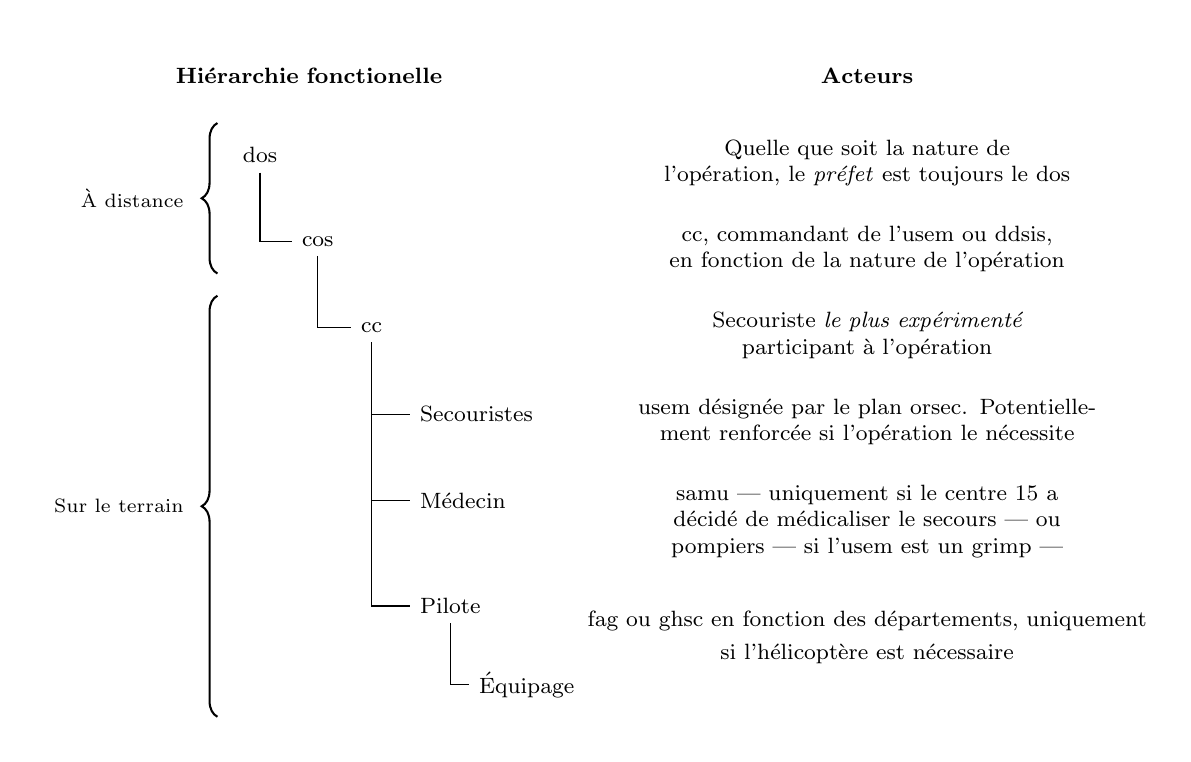
\begin{tikzpicture}
\usetikzlibrary{matrix, fit}
\usetikzlibrary{decorations.pathreplacing, calc}

\tikzset{ 
  table/.style={
    matrix of nodes,
    nodes={align=center, font=\footnotesize,  minimum height=10mm},
    nodes in empty cells,
    column 1/.style={nodes={text width=19em}},
    column 2/.style={nodes={text width=20em}}
  }
}

% Tableau
\matrix (m) [table] {
  % Ligne supérieure du tableau
  \toprule
  % Titre, en gras
  {\bfseries Hiérarchie fonctionelle} & {\bfseries Acteurs} \\
  \midrule
  % Pas de colonne 1, remplie après
  &Quelle que soit la nature de l'opération, le \emph{préfet} est
  toujours le \ac{dos}\\
  &\ac{cc}, commandant de l'\ac{usem} ou \ac{ddsis}, en fonction de
  la nature de l'opération\\
  &Secouriste \emph{le plus expérimenté} participant à l'opération\\
  &\ac{usem} désignée par le  plan \ac{orsec}. Potentiellement renforcée si l'opération le nécessite\\
  &\ac{samu} ---~uniquement si le centre 15 a décidé de médicaliser
  le secours~--- ou pompiers ---~si l'\ac{usem} est un
  \ac{grimp}~---\\
  % Lignes vides pour le multirow
  &\\
  &\\
};

% Texte centré sur les deux dernières lignes
\node[fit=(m-7-2)(m-8-2)]{\footnotesize \ac{fag} ou \ac{ghsc} en
  fonction des départements, uniquement si l'hélicoptère est
  nécessaire};
  
% Génération de l'arbre en colonne 1
\node[anchor=west](dos) at
([xshift=2.5cm]m-2-1.west){\footnotesize\ac{dos}};
%
\node[anchor=west](cos) at ([xshift=3.25cm]m-3-1.west)
{\footnotesize\ac{cos}};
%
\node[anchor=west](cc) at ([xshift=4cm]m-4-1.west)
{\footnotesize\ac{cc}};
%
\node[anchor=west](sec) at ([xshift=4.75cm]m-5-1.west)
{\footnotesize Secouristes};
%
\node[anchor=west](med) at ([xshift=4.75cm]m-6-1.west) {\footnotesize
  Médecin};
%
\node[anchor=west](heli) at ([xshift=4.75cm]m-7-1.west) {\footnotesize
  Pilote};
% 
\node[anchor=west](equi) at ([xshift=5.5cm]m-8-1.west) {\footnotesize
  Équipage};
% Arcs de l'arbre
\path[draw] (dos) |- (cos);
\path[draw] (cos) |- (cc);
\path[draw] (cc) |- (sec);
\path[draw] (cc) |- (med);
\path[draw] (cc) |- (heli);
\path[draw] (heli) |- (equi);

% Accolades
\draw [decorate,decoration={brace,amplitude=.2cm,
  raise=.2cm,mirror},line width=.75pt]
([xshift=2.5cm,yshift=-.1cm]m-2-1.north west) --
([xshift=2.5cm,yshift=.1cm]m-3-1.south west) node[midway, left,
xshift=-.5cm] {\scriptsize À distance};
%
\draw [decorate,decoration={brace,amplitude=.2cm,
  raise=.2cm,mirror},line width=.75pt]
([xshift=2.5cm,yshift=-.1cm]m-4-1.north west) --
([xshift=2.5cm,yshift=.1cm]m-8-1.south west) node[midway, left,
xshift=-.5cm] {\scriptsize Sur le terrain};
\end{tikzpicture}
  \caption{Synthèse des acteurs participant aux opérations de secours}
  \label{tbl:org_sec}
\end{table}

\paragraph{Spécificités locales}

Chaque département pouvant organiser les secours avec une certaine
latitude, on retrouve quelques spécificités départementales. La
principale différence entre les départements sont les unités qui
participent aux secours. La plupart des départements alpins ont
recours a un système d'alternance hebdomadaire
(\autoref{tab:organisation_secours_departements}). Ce système n'est
pas nécessairement appliqué dans l'ensemble du département. Dans les
Hautes-Alpes, par exemple, trois cas spécifiques sont définis. Si le
secours a lieu en zone de haute-montagne ou de moyenne montagne
accessible uniquement par hélicoptère, le secours est à la charge de
l'\ac{usem} de permanence, située à Briançon. Dans le cas où la
victime est dans une zone de moyenne montagne facilement accessible le
secours est à la charge du \ac{gmsp} de Gap. Cette organisation permet
d'adapter le dispositif d’intervention à la topographie du
département, les zones de haute-montagne étant principalement situées
dans le briançonnais, au nord-est du département. D'autres
départements ont des organisations particulières. Dans les
Alpes-de-haute-Provence, par exemple, le secours en montagne est à la
charge seule du \ac{pghm} de Jausiers. Enfin, pour des raisons
historiques, le département de la Haute-Savoie est organisé suivant un
régime unique. Dans la majorité du département les secours sont
réalisés par une équipe mixte, toujours composée de secouristes du
\ac{pghm} et de pompiers du \ac{gmsp}. Mais les secours dans le massif
du mont Blanc, où les secours sont à la charge seule du \ac{pghm},
acteur historique des secours dans le département
\autocite{Halle2007,Boillot2017}.

\begin{table}
  \centering
  \begin{tabular}{L{6cm}L{8cm}}
  \toprule
  \multicolumn{1}{c}{\bfseries Départements} & \multicolumn{1}{c}{\bfseries Organisation} \\
  \midrule
  Hautes-Alpes (05), Alpes-Maritimes (06), Isère (38), Savoie (73) & Alternance hebdomadaire \ac{crsm}, \ac{pghm} (selon un calendrier national).\\
  Alpes de Haute-Provence (04) & \ac{pghm} uniquement.\\
  Haute-Savoie (74) & Collaboration \ac{pghm}, \ac{gmsp}, sauf dans la région de Chamonux (\ac{gmsp} uniquement) et dans le massif du Mont-Blanc (\ac{pghm} uniquement). \\
  \bottomrule
\end{tabular}
  \caption{Corps mobilisés pour le secours en montagne dans les
    départements alpins.}
  \label{tab:organisation_secours_departements}
\end{table}

% Répartition des hélicoptères
Une autre différence notable entre les départements est la nature des
moyens héliportés à la disposition des secouristes. Pour des raisons
historiques, les appareils destinés au secours en montagne sont
répartis entre deux acteurs, la \emph{sécurité civile} par le biais de
son \emph{groupement hélicoptère} \acp{ghsc} et la \emph{gendarmerie}
par le biais de sa \emph{force aérienne} \acp{fag}. Cette différence a
principalement des conséquences administratives, les \emph{Dragons} et
les \emph{Choucas} \footnote{\emph{Dragon} et \emph{Choucas} sont,
  respectivement, les indicatifs radio des hélicoptères du \ac{ghsc}
  et de la \ac{fag}. Ce dernier est généralement postfixé par le
  numéro du département de rattachement de l'hélicoptère, \eg
  \emph{Choucas 05,} \emph{Dragon 38.}} déployés en montagne
correspondant au même modèle d'appareil \footnote{Des
  \emph{EC145}.}. La répartition des hélicoptères est fixée au niveau
national. Certains départements n'ont accès qu'a un seul appareil,
comme les Hautes-Alpes et les Alpes-de-Haute-Provence (appareils des
\ac{fag}), d'autres à deux, comme l'Isère (deux appareils
duispell-regioc \ac{ghsc}), la Savoie et la Haute-Savoie (avec un
appareil des \ac{fag} et un du \ac{ghsc} par département). Dans les
cas où les secouristes ne peuvent pas réaliser un secours faute
d'hélicoptère (appareil déjà utilisé ou en panne), il leur est
possible de demander une assistance à un département voisin. En Isère,
par exemple, le plan \ac{orsec} préconise de faire cette demande si le
délai d'attente pour disposer d'un hélicoptère est supérieur à 30
minutes.
% Coordination entre départements
Ces modalités d'assistance intra-départementale sont directement
fixées par les préfets de départements et non directement au niveau
national. Cependant, la coopération intra-départementale doit toujours
s'effectuer sous la coordination du \emph{centre opérationnel de zone}
\acp{coz} \footnote{Lequel est placé sous l'autorité du préfet de
  zone.} qui coordonne les différents \ac{codis} concernés. Par
exemple, le prêt de l'hélicoptère du détachement haut-alpin de la
\ac{fag} (\emph{Choucas05}) doit se faire sous la responsabilité du
\ac{coz} Sud, dont dépend le département des Hautes-Alpes

\paragraph{Le cas isérois}

Dans le cas du département de l'Isère, les dispositions spécifiques au
secours en montagne du plan \ac{orsec} datent de 2016 et ont été
modifiées pour la dernière fois en 2018.

% Organisation Géographique
Comme dans les Hautes-Alpes, plusieurs zones d'interventions sont
définies. Le \emph{plan de secours en montagne} \acp{pms} ne
s'applique que dans la partie sud-est du département
(\autoref{crt:isere_psm}). Les interventions de secours en montagne
dans cette zone relèvent de la compétence exclusive des \ac{usem}, à
l'exception du secours sur \emph{domaines skiables,} conformément à la
réglementation nationale. De plus, certaines formes spécifiques de
secours en \emph{domaine montagne}, comme le secours spéléologique
\footnote{Des dispositions spécifiques au secours spéléologique sont
  définies dans le plan \ac{orsec}. Contrairement au secours en
  montagne, ce type de secours est toujours assuré par des bénévoles
  soutenus par des moyens étatiques.} ou routier \footnote{Assuré par
  le \ac{grimp} isèrois.}, ne relèvent pas des \ac{usem} isèroises.

\begin{figure}
  \centering
  \begin{tikzpicture}

  % Styles
  \tikzset{ caisson/.style={minimum width=1cm, minimum height=.5cm},
    legende/.style={xshift=-2.5mm, anchor=west, text width=5cm},
    etiquette/.style={anchor=base west, font=\tiny},
    route/.style={draw=black, line width=.12mm} }

  % Import figures
  \node[inner sep=0pt, anchor=south west] (image) at
  (0,0){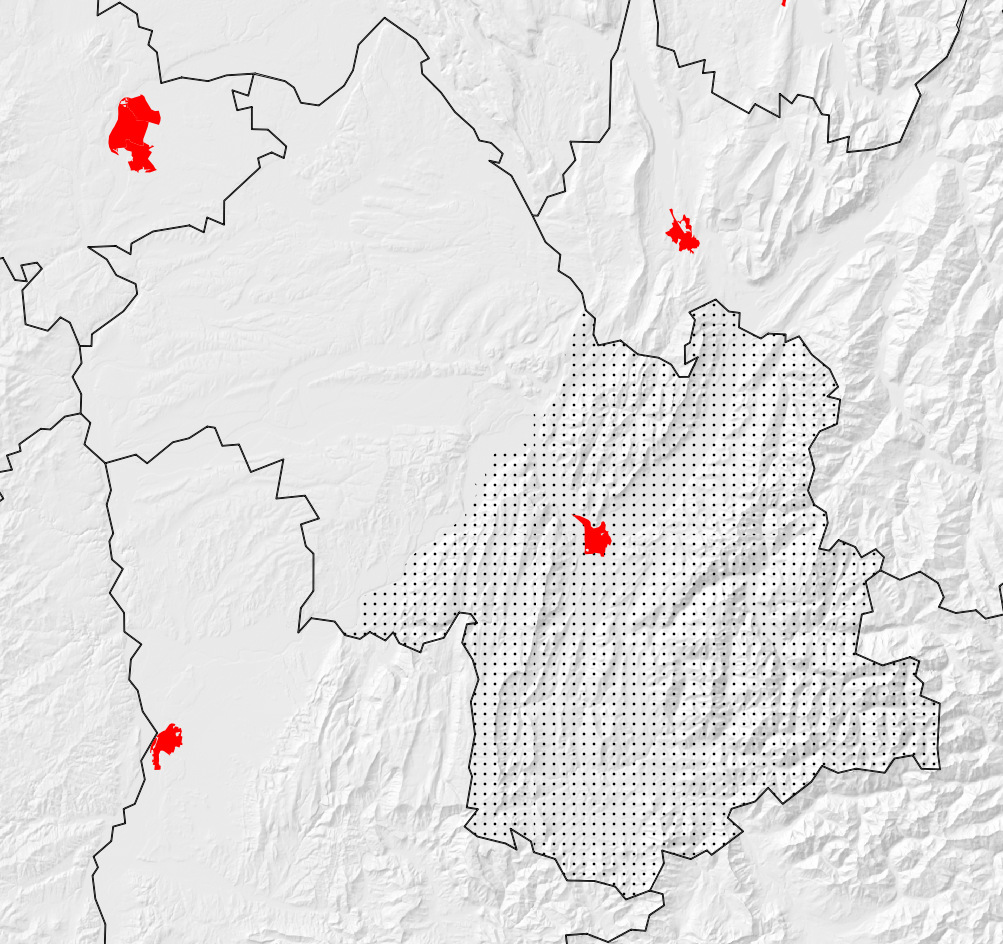
\includegraphics{./figures/Carte_PSM/Out1.png}};

  % \draw[help lines,xstep=.1,ystep=.1] (0,0) grid (image.north east);

  \begin{scope}
    \node[etiquette] (vs) at (5.55,3.85) {Le Versoud};
    \node[etiquette, anchor=base east] (ah) at (6.7,3.05) {L'Alpe d'Huez};
    \node[etiquette, anchor=base east] (bé) at (7.7,2.1) {La Bérarde};
  \end{scope}

  \begin{scope}
    \node (P2) at ([xshift=.5cm]image.south east) {};
    \node (P1) at ([xshift=.5cm]image.north east) {};

    % Légende
    \node (rect) [anchor=north west, caisson] at ([yshift=-2cm]P1) {};
    \path[route](rect.west) -- (rect.north) -- (rect.east);
    \node[right of=rect, legende] {\scriptsize Limies départementales};

    \node (rect) [anchor=north west, caisson, fill=red] at ([yshift=-2.75cm]P1) {};
    \node[right of=rect, legende] {\scriptsize Zones urbaines};

    \node (rect) [anchor=north west, caisson, pattern=dots] at
    ([yshift=-3.5cm]P1) {}; \node[right of=rect, legende] {\scriptsize
      Zone d'application du plan \ac{orsec}};

    \node (rect) [anchor=north west, caisson] at ([yshift=-4.25cm]P1)
    {}; \draw[anchor=north west, fill=RdBu-9-9, draw=none] (rect)
    circle [radius=0.1cm]; \node[right of=rect, legende] {\scriptsize
      Base permanente};

    \node (rect) [anchor=north west, caisson] at ([yshift=-5cm]P1) {};
    \draw[anchor=north west, fill=RdBu-9-8, draw=none] (rect) circle
    [radius=0.1cm]; \node[right of=rect, legende] {\scriptsize Bases saisonnières};

    % Échelle
    \draw[-] (P2 |- 1cm,0) --++ (1,0) node[pos=.5, above] {\footnotesize\SI{17.5}{\kilo\meter}};
  \end{scope}

\end{tikzpicture}
  \caption{Zone d'application des dispositions spécifiques au secours
    en montagne du plan \ac{orsec} en Isère.}
  \label{crt:isere_psm}
\end{figure}

% Acteurs dans le département
Les seules \ac{usem} présentes dans le département sont le \ac{pghm}
et la \ac{crsm}. Ces deux corps fonctionnent selon le principe
d'alternance hebdomadaire, commun à beaucoup de
départements. Cependant le plan \ac{orsec} départemental n’exclut pas
la participation occasionnelle d'autres acteurs, comme les pompiers,
les militaires du régiment grenoblois d’infanterie alpine, des unités
de la gendarmerie iséroise ou des bénévoles (généralement guides de
haute montagne).
% Opérateurs privés
La compagnie d'hélicoptères privées SAF participe également à des
opérations dans le département, notamment pour la station de l'Alpe
d'Huez qui fait évacuer certains blessés directement par hélicoptère.

% Adaptation du dispositif à la saison
Une autre particularité iséroise est l'adaptation du dispositif de
secours aux flux touristiques \footnote{Il ne s'agit cependant pas
  d'un cas unique. Un système similaire est également mis en place en
  Savoie.}. L'aérodrome du Versoud, en périphérie de Grenoble, est le
point central des opérations de secours. Un hélicoptère et son
équipage, une équipe de l'\ac{usem} d'astreinte et un médecin du
\ac{smur} y sont présents tout au long de l'année. Cette équipe est
complétée à la haute saison (été et hiver) par une seconde permanence
à l'altiport de l'Alpe d'Huez. Y sont présents, comme pour le Versoud,
un hélicoptère et son équipage, une équipe de secouristes et un
médecin. Enfin, durant l'été, une troisième équipe est déployée au
poste de secours de la Bérarde, point de départ d'un grand nombre de
randonnées dans l'Oisans et les Écrins. La mise en place de ces deux
permanences de haute-saison est néanmoins contrainte à une
disponibilité suffisante des moyens humains et matériels; si ceux-ci
ne sont pas suffisants, le maintient de la base du Versoud est
prioritaire.

\subsection{La phase de localisation des victimes}
\label{susec:1-1-2}

Jusqu'à présent nous avons traité les opérations de secours en
montagne comme \enquote{un tout}, sans en détailler l'organisation.
Pourtant la phase de \emph{traitement de l'alerte} et celle de
\emph{l'intervention} répondent à des objectifs et mobilisent des
compétences très différentes. C'est durant la phase de traitement de
l'alerte que sont fixées les modalités d'intervention, de
médicalisation et que la victime et sa position sont identifiées. Or,
si toute intervention nécessite de connaitre la position de la
victime, il n'est pas forcément simple ou rapide de l'identifier. Il
s'agit donc d'une étape critique, avec un impact conséquent sur
l'ensemble d'une opération de secours. La circulaire \bsc{Kihl} en
impose même la vérification systématique. Une erreur pouvant faire
perdre un temps considérable aux équipes de secours et donc impacter,
non seulement l'opération de secours en cours, mais également toutes
les opérations ultérieures, les moyens nécessaires aux secours étant
limités.

% Organisation de la recherche de victimes en Isère
Dans le département de l'Isère, ce travail de localisation de la
victime est à la charge des \ac{usem}. En effet, le plan \ac{orsec} de
l'Isère précise que \enquote{l’opération de secours \textelp{} englobe
  la phase de localisation précise de la victime \textelp{}}
\footnote{\emph{Les principes du secours en montagne en Isère,} page 5
  du plan \ac{orsec} de l'Isère.} et que, en vertu du principe de
\enquote{compétence exclusive} des \ac{usem} pour les opérations de
\emph{secours en montagne,} la localisation de la victime est à leur
charge.

\subsubsection{L'identification manuelle de la position des victimes}
\label{subsec:1-1-2-1}

Les secouristes disposent de plusieurs méthodes pour localiser les
victimes. Une première manière de procéder, qui nous intéresse
particulièrement dans le cadre de ce travail, consiste à identifier
manuellement la position du requérant à partir des informations de
localisation données lors de l'appel, \eg \enquote{Je suis sur le
  GR~5}, \enquote{Je vois Grenoble} ou \enquote{Je suis à côté d'un
  chalet.} Ces informations peuvent être extrêmement nombreuses et
précises ou, au contraire, extrêmement lapidaires. L'identification
manuelle d'une position peut donc être un travail difficile, même pour
un secouriste habitué a ce travail.

Le processus de localisation d'une victime par les secouristes est
unique dans chaque cas, mais on peut identifier certaines
récurrences. Lorsque la personne contactant les secours, \emph{le
  requérant,} est mise en contact avec les secouristes il lui est
rapidement demandé de donner sa position. Quelques fois le requérant
est capable de la donner précisément et sans ambiguïtés, par exemple
en donnant des coordonnées GPS ou une indication extrêmement claire et
discriminante (\eg \enquote{Je suis au sommet du Grand Veymont}). Mais
dans la majorité des situations le requérant n'est pas capable de
décrire convenablement sa position. Les secouristes doivent donc
l'identifier, ou tout du moins l'approximer à partir des informations
qu'ils peuvent obtenir. Cette tâche est cependant facilitée par deux
éléments importants. D'une part, la phase de localisation se déroule
en parallèle de la conversation téléphonique entre le requérant et un
secouriste. Ce dernier n'a donc pas à extrapoler le maximum
d'informations à partir d'une description figée, au contraire, il a la
possibilité de poser des questions, de demander des précisions et donc
de tester des hypothèses. Les secouristes peuvent donc procéder par
essais-erreurs et adapter leur démarche en continu, en fonction de la
situation et des nouvelles informations données par le requérant, ce
qui facilite le travail de localisation. Le second point essentiel,
est que les secouristes peuvent s'appuyer sur un nombre conséquent de
données pour identifier la position du requérant. En effet, les
secouristes ont accès à un ensemble de données cartographiques, que ce
soit au format papier ou numérique, qui leur permettent d'identifier
des positions, de faire des hypothèses ou de poser des questions
discriminantes (\eg \enquote{Est-ce que vous voyez des chalets au loin
  ?}). D'autres sources d'informations sont également disponibles pour
les secouristes, comme un ensemble de \emph{topo-guides}
\footnote{Guides pour les courses en montagne.} de la région, dans
lesquels sont parfois les seuls documents à donner une information
spécifique, comme un itinéraire recommandé.

% Les trucs qui compliquent
Malgré ces atouts, il est parfois difficile pour les secouristes
d'identifier avec précision et certitude la position de la victime,
notamment lorsque les informations données par le requérant sont peu
précises ou vagues. Cela peut se produire lorsque le requérant est un
tiers contactant les secouristes suite à une disparition ou lorsque la
victime est complètement perdue, paniquée ou gravement blessée.

\paragraph{Le cas spécifique des \emph{domaines skiables}}

Il convient de préciser que le processus d'identification des
positions est assez différent lorsque les \ac{usem} sont amenées à
intervenir sur un \emph{domaine skiable.} Dans ce cas, les victimes ne
contactent pas directement les secouristes des \ac{usem}
\footnote{Conformément au plan \ac{orsec} les appels adressés au
  \ac{codis} (112 ou 18) ou au \ac{samu} (15) pour des secours sur
  \emph{domaine skiable} sont redirigés au service des pistes
  concerné.}, ce sont les \emph{pisteurs-secouristes} de la station
qui prennent contact avec le \ac{codis} pour demander une évacuation
héliportée si la situation l'impose.

Dans cette situation la communication est donc assez différente,
puisqu'elle s'effectue entre deux professionnels, qui partagent des
connaissances sur la région de l'intervention et qui sont
régulièrement amenés à communiquer entre eux. Des solutions techniques
ont donc étés mises en place pour faciliter et fluidifier ces
interactions. D'une part les secouristes de \ac{usem} ont accès à
l'ensemble des plans de piste des \emph{domaines skiables} de leur
zone d'intervention, complétés par carroyage commun entre
\emph{pisteurs-secouristes} et \ac{usem}. Ce dernier permet aux
pisteurs de communiquer rapidement une position aux secouristes, bien
plus qu'avec une description.  Les problèmes pouvant apparaitre lors
de la localisation manuelle des victimes sont donc inexistants dans le
cas particulier des secours en station de ski, c'est pourquoi nous ne
traiterons pas de ce cas dans notre thèse.

On peut toutefois noter que la solution développée par les secouristes
et les pisteurs n'est pas exempte de défauts. Pour des raisons autant
pratiques qu’esthétiques, les plans de stations de ski sont fortement
déformés, voir peu réalistes pour ceux dessinés manuellement
\autocite{Gauchon2014,LaPorte2017}. Tout carroyage tracé sur ces
représentations est donc difficilement transposable dans une
représentation azimutale, comme une carte topographique ou un
\ac{sig}, ce qui impose aux secouristes ou aux pilotes de faire cette
transformation mentalement. Au sein du projet Choucas plusieurs
travaux d'étudiants ont été mis en place pour permettre le
géoréférencement de ces plans et donc faciliter leur utilisation
\autocite{Gauer2019,Xi2020}.

\subsubsection{L'identification assistée de la position de la victime}
\label{subsec:1-1-2-2}

Lorsque la victime contacte directement les secours (ou que le
requérant est présent sur le site de l'accident) le processus de
localisation peut être assisté par l'utilisation de solutions
permettant une géolocalisation facile, précise et non ambiguë (\eg
comme les récepteurs GPS). La généralisation des smartphones, qui en
sont majoritairement équipés, a fait émerger un marché de solutions de
partage de localisation pensées pour le secours. Les applications
dédiées, comme \emph{Alpify,} sont peu à peu supplantées par les
solutions directement intégrées dans le système d'exploitation des
appareils, comme le système \emph{Android Emergency Location Service}
\autocite{Google2019}. De telles solutions sont certes utiles, mais
elles ne sont que des aides occasionnelles, totalement dépendantes de
la victime et de sa capacité a les utiliser. Il existe cependant deux
solutions que les secouristes peuvent utiliser a leur initiative,
l'identification de l'antenne GSM servant à passer l'appel et
l'application de géolocalisation \emph{Gend'Loc.}

\paragraph{L'identification de l'antenne GSM}

Les \ac{usem} ont la possibilité de localiser le requérant en
identifiant l'antenne GSM à laquelle son téléphone est connecté. Le
principal avantage de cette méthode est qu'elle est totalement
transparente pour la victime. Aucune action de sa part n'est
nécessaire pour la localiser. Toutefois c'est le seul avantage de
cette méthode, qui n'est ni précise, ni rapide.

D'une part cette approche ne renseigne les secouristes que sur
l'antenne téléphonique de rattachement et sur son angle d'émission, le
requérant peut donc se situer n'importe où dans la zone couverte par
l'antenne. Or, lorsque que le maillage est composé d'un faible nombre
d'antennes puissantes, comme c'est généralement le cas en dehors des
milieux urbains, la zone couverte par l'antenne peut devenir très
importante (\ie atteindre plusieurs centaines de km\up{2}) et donc ne
pas permettre une localisation suffisamment précise. À cela s'ajoute
le fait que la zone couverte par une antenne peut varier sensiblement,
notamment en fonction des conditions météo, ce qui renforce
l'imprécision de la localisation par ce biais
\autocite{FenChong2012,OlteanuRaimond2012}.

À la faible précision de cette méthode s'ajoute sa lenteur. Pour des
raisons légales les secouristes ne peuvent obtenir cette information
des opérateurs qu'avec une réquisition judiciaire. La demande de cette
réquisition n'est pas automatique, il est donc nécessaire de faire une
demande manuellement, d'attendre sa validation avant de contacter
l'opérateur du requérant qui renverra l'information
demandée. L'ensemble de ce processus peut donc prendre plusieurs
dizaines de minutes, ce qui, dans un contexte d'urgence et de
ressources matérielles limitées, est considérablement long.

Dans les faits, l'identification de l'antenne GSM utilisée par le
requérant n'est que rarement employée par les secouristes. Les
secouristes ont généralement recours a cette solution lorsque aucune
des informations données par le requérant n'est suffisante pour le
localiser, que la phase de localisation prend beaucoup de temps et que
l’application \emph{Gend'Loc} n'est pas utilisable.

\paragraph{La solution \emph{Gend'Loc}}

Pour disposer d'une aide à la localisation plus rapide, précise et
efficace que l'identification de l'antenne GSM utilisée, les
secouristes du \ac{pghm} de Grenoble ont développé, à partir de 2013,
l’application \emph{Gend'Loc.} Contrairement a une application pour
smartphone ---~comme celle \footnote{Cette application, qui s’appelait
  auparavant \emph{IRera,} porte aujourd'hui le nom de \emph{Rega.}}
proposée par la Garde aérienne suisse de sauvetage (REGA)~---
\emph{Gend'Loc} ne demande pas un téléchargement et une installation
préalable. Le principe de fonctionnement de \emph{Gend'Loc} consiste à
envoyer, par SMS, une URL au requérant. Cette dernière conduit à une
page web \emph{ad hoc,} qui demande, par le biais du navigateur web,
la localisation du téléphone. Si la victime valide l'opération, la
position du téléphone est automatiquement renvoyée aux secouristes,
qui peuvent l'afficher directement à l'aide d'une interface
cartographique \emph{ad hoc.}  Avec cette solution les secouristes
peuvent connaitre rapidement et précisément la position de la victime,
sans qu'il soit nécessaire de passer par une autorité judiciaire, ce
qui facilite grandement les opérations de secours
\autocite{Muscat2015}. Un second avantage de cette solution, est
qu'elle offre la possibilité de guider des personnes perdues, mais non
blessées, sans qu'il soit nécessaire d'effectuer une intervention. En
effet, \emph{Ged'Loc} permet de générer un plan centré sur la position
de la victime et de lui transmettre. Ce qui permet généralement à la
victime de retrouver son chemin \autocite{Muscat2015}.


Ce paragraphe devrait être re-travailler; Je vois deux améliorations :
1/ enlever tout ce qui compare cette solution à la localisation à
l'antenne 2/ en mieux listant les limites : - pas de smartphone - pas
de réseau 4 G, ou mauvaise connexion - pas assez de batterie pour
activer le GPS; dans ce cas, le PGHM demande aux victimes de ne rien
faire; afin que le téléphone reste allumé; - le requérant n'est pas la
victime - la victime n'est pas en mesure de faire les manipulations
demandées à cause des blessures;

%Les limites de la solution
Bien qu’extrêmement efficace cet outil ne peut pas apporter de
solution satisfaisante à toutes les situations. Son principal défaut
est sa dépendance aux smartphones et a leur GPS intégré. Si la
majorité des Français possède aujourd'hui ce type de téléphone
\footnote{Plus précisément 77 \% en 2019, selon le baromètre de
  l'\textcite{ARCEP2019}.} cette répartition présente une forte
hétérogénéité inter-classes d'age \footnote{86 \% des 12-17 ans
  possèdent un \emph{smartphone,} contre 98 \% des 18-24 ans, 95 \%
  des 25-39 ans, 80 \% des 40-59 ans, 62 \% des 60-69 ans et 44 \% des
  70 ans et plus, selon le baromètre de l'\textcite{ARCEP2019}.}. Par
conséquent, une part, sans doute minoritaire, mais non négligeable des
requérants n'a pas accès à un GPS, ce qui rend leur géolocalisation
impossible à l'aide de \emph{Gend'Loc} \footnote{À cet égard la
  solution proposée par \emph{Gend'Loc} est moins flexible que
  l'identification des antennes GSM. En effet, cette solution permet
  connaitre la position de n'importe quel téléphone portable, qu'il
  ait un GPS ou non.}. De plus il est nécessaire que la victime ait
une connexion mobile d'assez bonne qualité pour pouvoir accéder à
internet et donc ouvrir la page web transmisse par \emph{Gend'Loc.}
Enfin, il est nécessaire que la victime puisse réaliser l'ensemble des
manipulations nécessaires \footnote{%
  \begin{enumerate*}[label=(\arabic*)]
  \item Ouvrir le lien donné par SMS,
  \item allumer le GPS du téléphone,
  \item autoriser le navigateur à transmettre la position du GPS, et
  \item valider le partage de la position sur la page web \emph{Gend'Loc.} 
  \end{enumerate*}}.
%
Or, la victime peut être dans de semi-lucidité ou de panique qui
l’empêche de les réaliser convenablement. Les secouristes du \ac{pghm}
de Grenoble nous ont indiqué qu'ils choisissaient fréquemment de ne
pas utiliser \emph{Gend'Loc} dans ces conditions, préférant rester en
contact avec la victime, quitte à identifier sa position manuellement.

\subsubsection{Le cas \enquote{\emph{fil rouge}}}
\label{subsec:1-1-2-3}

Il existe cependant certaines situations où, malgré les outils de
géolocalisation, la localisation des victimes est délicate. C'est par
exemple le cas du \emph{fil rouge,} une opération de secours en
montagne qui s'est déroulée en aout 2014, dans la région de
Bourg-d'Oisans, en Isère (\autoref{crt:fil_rouge}). Un randonneur,
polytraumatisé suite à une chute, contacte les secours et est mis en
relation avec le \ac{pghm} de Grenoble. Son état étant assez
préoccupant, le secouriste en fonction l'estime incapable d'utiliser
\emph{Gend'Loc,} l'identification de sa position se fait donc
manuellement, par recoupement d'informations.

\begin{figure}
  \centering
  \begin{tikzpicture}
  \tikzset{et/.style={above,font=\footnotesize\vphantom{Ag}}}
  % 
  \node[inner sep=0pt, anchor=south west] (image) at (0,0){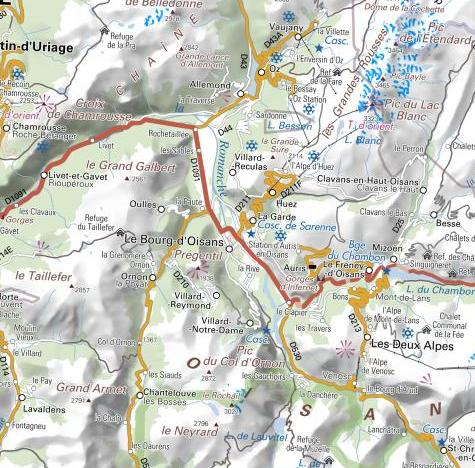
\includegraphics{./figures/bourdOisans.jpg}};
  % 
  \begin{scope}
    \node (P2) at ([yshift=-.5cm]image.south east) {};
    \node (P1) at ([yshift=-.5cm]image.south west) {};
    % Échelle
    \draw[-] (P2 |- -1cm,-1cm) --++ (-1,0) node[et,pos=.5] {\SI{2,500}{\kilo\meter}};
    % Légende détaillée
    \path (P1) -- (P2) node[pos=.5, yshift=-2.5cm] {\tiny Source:
      Géoportail, SCAN régional IGN, 2020.};
  \end{scope}
\end{tikzpicture}
  \caption{Région de Bourg-d'Oisans}
  \label{fig:fil_rouge}
\end{figure}

Toutefois la victime n'est pas toujours lucide et les informations que
les secouristes obtiennent, en quarante minutes de conversation, sont
peu nombreuses et précises. Au cours de la conversation les
secouristes obtiennent de la victime les informations suivantes :

\begin{itemize}
\item Elle est partie de Bourg d'Oisans, à pied, sur chemin, en
  direction d'une station de ski.
\item Elle a marché plusieurs heures.
\item Elle a chuté de plusieurs mètres.
\item Elle voit une partie de plan d'eau.
\item Elle est sous une route et entend des véhicules.
\item Elle est sous une ligne électrique 3 brins.
\item Elle vient de passer du soleil à l'ombre.
\end{itemize}

La particularité de cette alerte est que toutes les informations
données par le requérant sont imprécises et donc difficiles à
utiliser. Le seul lieu nommé (et donc facilement identifiable) est le
point de départ de la victime. Les autres éléments de localisation
donnés par la victime le localisent par rapport à un type d'objet. On
sait par exemple que la victime s'est dirigée vers une station de ski,
mais sans savoir laquelle. De plus, toutes les informations qui
permanenteraient d'identifier la position actuelle à partir du point
de départ sont imprécises, \enquote{quelques heures},
\enquote{plusieurs mètres}, etc. Par conséquent, plusieurs endroits
dans la région de Bourg-d'Oisans correspondent à cette
description. Les secouristes complètent donc leurs informations avec
une réquisition auprès de l'opérateur de téléphonie mobile, ce qui
leur apporte une nouvelle information, le téléphone de la victime est
connecté à une antenne \enquote{GSM SFR située à la chapelle
  st-Philomene à Villard-Reymond (\num{38520}) et orientée au 90°}
\autocite{Lot 0.4}. Cette nouvelle information permet de réduire
suffisamment la zone de recherche pour que les secouristes prennent la
décision d'envoyer un hélicoptère pour chercher la victime de visu,
avant que le soleil ne se couche.
% Conclusion
La victime est finalement repérée par l'équipage de l'hélicoptère en
vol. De l'aveu même des secouristes la réussite de cette opération de
secours tient beaucoup à la chance et leur difficulté à résoudre ce
cas les a amenés à réfléchir à de nouvelles pistes d'amélioration de
leur méthodologie.

%%% Local Variables:
%%% mode: latex
%%% TeX-master: "../../../../main"
%%% End:
